\chapter{Concept and Design}
\label{cha:conceptanddesign}


\section{Big Picture}

As already mentioned our system consisted of two parts, the mobile clients side and the backend side which interconnectedly exchanged data. The backend part itself was split up again in three parts of which one was an \enquote{external} (means: SNET) resource, the CYCLONE Federation Provider. This entity provided us with user management and session handling functionalities so that we were able to out source these tedious and error-prone tasks to them. On the other side CYCLONE profited from our experiences with its rather young service. Concerning our part of the backend side, the task was to serve two machines independently, the API server and the database server. This was expected to be achieved with Docker.

To gain an understanding of what system we were trying to build, the following image should be at help:

\begin{center}
    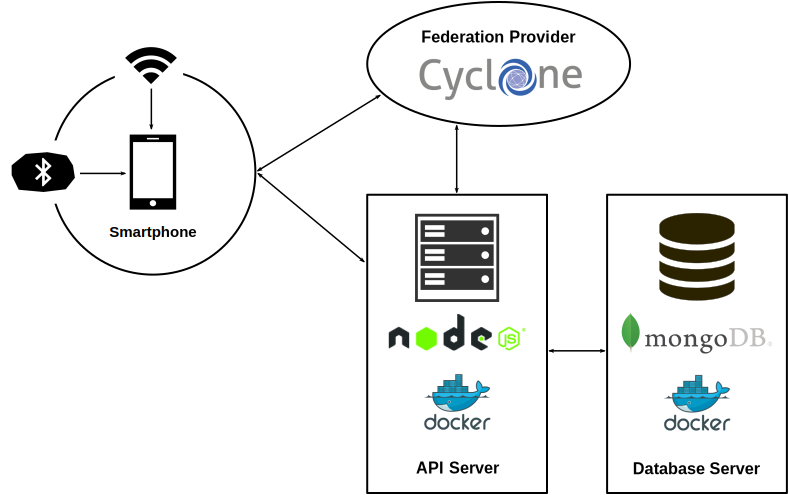
\includegraphics[width=\textwidth]{system-overview}\\
    All components of our envisioned system working together.
\end{center}

To sum it up, the idea was to gather position information aligned to the user's preferences locally on the smartphone, preform some processing steps on it, contact our backend for which authentication via the CYCLONE Federation Provider is needed and after that create, read, update or delete information (CRUD principle\footnote{\url{https://en.wikipedia.org/wiki/Create,_read,_update_and_delete}}) in the backend and therefore in the database.


\vspace{0.5cm}

\section{API Considerations}

We had to decide on which paradigm our API should be based on. With the client-server and stateless nature of our envisioned system setup in combination with the just mentioned approach of relying on HTTP verbs such as POST, GET, PUT and DELETE for the CRUD operations, the decision to go for a RESTful API was quite clear (\cite{fielding2000architectural}, chapter 5).

Furthermore a widely supported and light-weight format for interchanging data between clients and backend was needed, and it was decided to use JSON\footnote{\url{http://json.org/}}. This also played nicely together with our requirement to implement the API server in Node.JS\footnote{\url{https://nodejs.org/en/}}, using the Express web framework\footnote{\url{http://expressjs.com/}} which provided us a convenient way to define the RESTful resources of our API.


\vspace{0.5cm}

\section{Workload Split Between Clients and Server}


\vspace{0.5cm}

\section{Authentication and Session Management}

The CYCLONE Federation Provider provided us with the ability to integrate a well-tested user authentication method with only little effort into our service. CYCLONE is based on the JBoss Keycloak\footnote{\url{http://keycloak.jboss.org/}} project which in turn is based on the OpenID Connect standard\footnote{\url{https://openid.net/connect/}}, OAuth 2.0\footnote{\url{http://oauth.net/2/}}, JSON Web Token\footnote{\url{https://jwt.io/}} and SAML 2.0. In the following a short overview of the involved technologies will be given.

The OpenID Connect standard provides two important functionalities in focus of our project. The first one is the addition of an identity layer on top of the OAuth 2.0 Authorization Framework that enables developers to reliable verify what person is using the authenticated service, no matter the used client, be it web or native applications. OpenID Connect does this without the need to maintain password storages on developers' side. Specifically, the CYCLONE Federation Provider uses the Authorization Code Flow\footnote{\url{https://openid.net/specs/openid-connect-core-1_0.html\#CodeFlowAuth}} of the OpenID Connect standard. The other feature OpenID Connect brings into the project is that it already is built as a RESTful HTTP API based on JSON as the transport format and therefore perfectly integrated into the implementation and also provides the functionality to extend the specification in order to, for example, encrypt the transported identity data.

The OAuth 2.0 Authorization Framework is an IETF RFC \cite{hardt2012oauth} which introduces an abstraction layer, the authentication layer, in distributed web application environments. Therefore the standard is designed for the HTTP protocol and does not specify other protocols. OAuth 2.0 provides the ability to differentiate between resource owners (e.g. end users on a service, the resource server) and requesting third parties that need access to some or all resources of the resource owner. Third parties will never need to be authenticated by the resource owner's own credentials but will instead request an access token issued for specific scope, access duration and further attributes from an authorization server. This flow lets the resource owner be in full control of all allowed access requests from third parties, enabling her/him to eventually revoke granted access. Furthermore the attack vector on each involved participants in the service is isolated by separating all authorizations via the access tokens. An extensive threat model analysis on OAuth 2.0 can be found in \cite{lodderstedt2013oauth}.

JWTs (pronouned: \enquote{jots}) are another IETF RFC \cite{bradley2015json} standardizing the transfer of a set of claims as a JSON object in a compact and URL-safe manner. The standard defines three parts of an JWT with the first one being the algorithm and token part, the second being the payload and the third used to verfiy the transported JWT. Encoding and concatenating these fields with dots yields the mentioned URL-safe representation predestined to be transported in HTTP Authorization headers or URI query parameters.

This authentication environment helped us to achieve multiple goals in our implementation. First of all users were able to authenticate via their university account as it is part of the edugain collaboration for which CYCLONE acts as an federation provider. Therefore we had a single-sign-on mechanism available by simply integrating CYCLONE. The other major advantage was that we never saw the user's credentials used to authenticate. We were able to rely on the well-tested user authentication code base provided implicitely through the layered mechanisms the CYCLONE Federation Provider contained.


\vspace{0.5cm}

\section{Database Design}